% !TEX program = lualatex
% !TEX options = -lualatex

\documentclass{uetgraduation}

% --- Gói cần thiết (tùy chỉnh lại nếu cần) ---
\usepackage{needspace}
\usepackage{enumitem}
\usepackage{tabularx}
\usepackage{ltablex}
\keepXColumns
\usepackage{array}
\usepackage{makecell}
\usepackage{multirow}
\usepackage[hidelinks]{hyperref}
\usepackage{xurl}
\urlstyle{same}
\usepackage{seqsplit}
\usepackage{unicode-math}
\setmathfont{Cambria Math}
\usepackage{caption}
\usepackage{listings}
\usepackage{subfiles}

% --- Thông tin trang bìa ---
\begin{document}

% Trang bìa 1
\studentname{23020122 -- Phùng Hải Nam}
\studentnametwo{23020019 -- Nguyễn Văn Cường}
\studentnamethree{23021724 -- Tô Quang Thắng}
\title{Phát triển ứng dụng di động}
\documenttype{Báo cáo Phản biện ứng dụng Humble của nhóm Quýt}
\major{Công nghệ thông tin}
\year{2025}
\supervisor{TS. Nguyễn Đức Anh}
\cosupervisor{ThS. Trần Mạnh Cường}

\makecovers
% Mục lục
\begin{contentlisting}
    \begin{contentlistingsection}{}
        \listoftables
    \end{contentlistingsection}

    \begin{contentlistingsection}{}
        \listoffigures
    \end{contentlistingsection}
    \tableofcontents
\end{contentlisting}
\chapter{Phần báo cáo}
\begin{itemize}
    \item Căn lề lỗi: Hiện tại căn lề trái phải là dễ thấy lỗi nhất. Do thầy yêu cầu bám theo khóa luận tốt nghiệp, các bạn có thể tham khảo các quy định về căn lề để sửa chính xác hơn. (Tham khảo 1 vài mẫu khóa luận sẽ thấy lề trái phải cần được căn lệch chứ không căn đều)
    \item Cỡ chữ: Không tính những phần phụ như tên nhóm, tên thành viên (những phần không nằm trong mẫu khóa luận) thì cỡ chữ cũng đang bị sai ở trang bìa
    \item Đánh số trang cần bỏ các số trang la mã ở các trang trước phần mở đầu.
    \item Giãn cách dòng sai không thống nhất, có thể là do dùng shift enter với enter nhầm. Ví dụ: (Nhìn khoảng cách giữa dòng 1 với dòng 2 so với dòng 2 với dòng 3)
      
    \begin{figure}[H]{Một số ví dụ về lỗi giãn cách dòng}
        \centering
        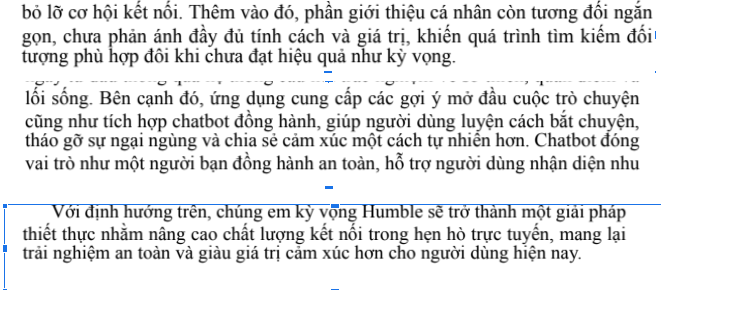
\includegraphics[width=\textwidth]{anh/vidu.png}
            
    \end{figure}
    \item Sơ đồ ca sử dụng chưa có biên hệ thống
    \item Sơ đồ ca sử dụng to nhỏ khác nhau các ca sử dụng
    \item Biểu đồ CSDL có các đường liên hệ chưa nối đúng trường khóa ngoại với trường tham chiếu tương ứng. Nhiều bảng có nhiều hơn 1 trường FK nhưng chỉ thấy 1 đường nối quan hệ
    \item Biểu đồ tuần tự chưa có thanh kích hoạt (activation bar).
    \item Bảng kiểm thử chức năng chưa có người kiểm thử, ngày kiểm thử, đầu ra thực tế và trạng thái kiểm thử (đạt/không đạt). Chữ trong bảng đôi khi còn bị tràn ra ngoài ô.
    \item Lỗi chính tả 
    \begin{figure}[H]{Ví dụ về lỗi chính tả}
        \centering
        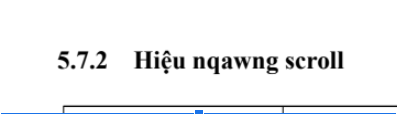
\includegraphics[width=\textwidth]{anh/chinhta.png}
            
    \end{figure}
    \item Sắp xếp thuật ngữ, trích dẫn theo bảng chữ cái.
    \item Xem lại cách trích dẫn theo tài liệu quy định 
\end{itemize}
\chapter{Phần mã nguồn}
\begin{itemize}
    \item apikey lộ
    \item không đề cập tới jetpack compose dù code UI dùng cái này
    \item code kotlin là chính chứ k phải java (sai so với báo cáo), jetpack compose tức là dùng kotlin
    \item “Tếp theo”: bị sai chính tả trên rất nhiều nút giống nhau mà không nhận ra (ảnh ở trong pdf và test thực tế vẫn bị sai)
    \item email xác nhận đăng ký flow không rõ ? nhận mail nhưng mail đi vào hòm thư rác, tên app trong mail chưa có, nhấn vào thì được điều hướng tới ảnh dưới, nhưng app thì không điều hướng gì cả, 
    nên cuối cùng không đăng ký được nên không chạy thử các giao diện còn lại trong hệ thống được. Hiện tại ngày 22/11 test bằng file release có sẵn trong repo.
\begin{figure}[H]{Ví dụ về giao diện}
    \centering
    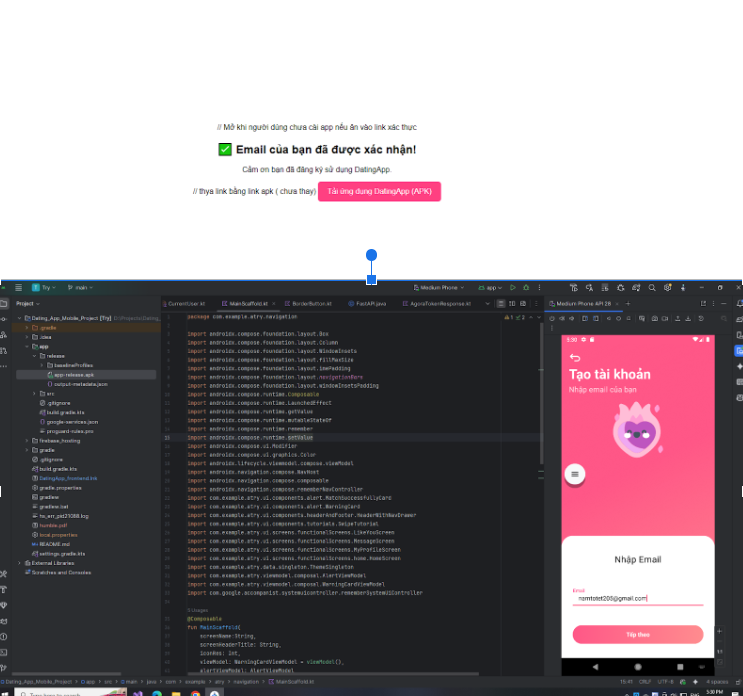
\includegraphics[width=\textwidth]{anh/saichinhta.png}
            
\end{figure}

\end{itemize}

\end{document}
